\section{Introducción}

Con el crecimiento de dispositivos inteligentes y las redes de alta velocidad, el Internet de las Cosas se ha convertido
en una tecnología con gran influencia, aceptación e impacto dentro de mercados del sector \cite{khan2018iot}. 

\vspace{5mm}

\noindent Ello representa una red interconectada donde dispositivos incorporados con sensores, están interconectados a 
través de una red privada o pública. Intercambiando datos comprometedores, críticos para la seguridad y protección, así 
como información sensible a la privacidad y, por lo tanto, son objetivos atractivos para diversos ciberataques 
\cite{dorri2017blockchain}. 

\vspace{5mm}

\noindent Un claro ejemplo fue el famoso ciberataque hacía el proveedor de DNS estadounidense Dyn. El ataque se originó 
de decenas de millones de direcciones IP, y que al menos parte del tráfico provenía de dispositivos IoT. Estos últimos 
habían sido infectados con un malware llamado Mirai, que se encargaba de controlar los dispositivos en linea y lanzar 
ataques de denegación de servicio distribuido (DDoS) \cite{kshetri2017can}. 

\vspace{5mm}

\noindent Los dispositivos IoT son limitados en cuanto a capacidad computacional, almacenamiento y conectividad, y en 
consecuencia son más vulnerables a ataques. Por ello, en este proyecto vamos a indagar, sobre cómo la tecnología 
emergente Blockchain, puede aportar beneficios con el objetivo de fortalecer la seguridad del Internet de las Cosas 
(IoT). Diversas compañias están tomando iniciativas para integrar la tecnología Blockchain en su produccción y 
suministro (p. ej., IBM, Cisco, Bosch, etc) \cite{kshetri2017can}.   

\subsection{Motivación} \label{motivacion}

La finalidad de este proyecto es realizar una labor de investigación sobre la tecnología Blockchain, su funcionalidad, 
tipos de herramientas y capacidades de desarrollo. Para elaborar un prototipo funcional de infraestructura distribuida 
de gestión de dispositivos IoT (Rapsberry Pi) dentro de una red domótica local \cite{huh2017managing}. La arquitectura 
distribuida asegurará la comunicación y sincronización de los datos entre los dispositivos, con el fin de llevarlo a 
dominios que están adaptando la tecnología IoT en sus labores de negocio.

\vspace{5mm}

\noindent Todo ello regido por contratos inteligentes para permitir realizar cualquier operación, de una forma segura, 
inmutable y trazable de los dispositivo dentro de la red.

\vspace{20mm}

\noindent Como prueba de concepto, se utilizarán 5 Raspberry Pi: 

\begin{itemize}
	\item 3 Raspberries Pi 4 Modelo B+ 2GB, que servirán como nodos principales de la red Blockchain.
	\item 2 Raspberry Pi 2 Modelo B+ que tomará el papel del actuador y un sensor (Raspberry Pi 3 Modelo B+), ambos 
	para simular la red domótica.
\end{itemize}

\noindent La configuración, establecida por el usuario, se encargará de indicar políticas entre los sensores 
y actuadores. El primero recogerá los valores del entorno y el otro efectuará la acción pertinente. Así por ejemplo, 
el sensor puede detectar una temperatura determinada dentro de la habitación, y en el caso de que sobre pase un 
umbral, se mandaría una señal al actuador, para encender el aire acondicionado. \cite{huh2017managing}

\vspace{5mm}

\noindent Entonces, todos los registros que se han llevado a cabo, se introducirán en la red Blockchain, haciendo que 
los datos sean inmutables, donde se podrán ver toda la trazabilidad de las transacciones que se han aceptado en la red 
de forma satisfactoria hasta el momento.

\subsection{Objetivos}

Los objetivos del trabajo son los siguientes:

\begin{itemize}
    \item Realizar un estudio de la tecnología Blockchain y el papel que puede tomar en el escenario del Internet de 
    las cosas, a nivel de soluciones, beneficios y desafíos \cite{khan2018iot, reyna2018blockchain}. 
    \item Seleccionar las herramientas existentes en el mercado para desarrollar la infraestructura, y la propia 
    aplicación.
    \item Elaborar un prototipo para implementar una red distribuida de gestión de dispositivos IoT y una aplicación
    para su gestión.
\end{itemize}

\newpage

\subsection{Introducción al Blockchain. Bitcoin}

El Bitcoin fue inventado en 2008 por Satoshi Nakamoto, que combinó la tecnología b-money\footnote{B-money 
fue una de las primeras propuestas creadas por Wei Dai para un "sistema electrónico de dinero en efectivo anónimo y 
distribuido". \label{fnlabel}} y HashCash\footnote{Hashcash es un sistema de prueba de trabajo que se utiliza para 
limitar el spam de correo electrónico y los ataques de denegación de servicio, y más recientemente se ha dado a 
conocer por su uso en bitcoin (y otras criptodivisas) como parte del algoritmo de minería. Hashcash fue propuesto 
en 1997 por Adam Back. \label{fnlabel}} para crear un sistema completamente descentralizado de dinero  electrónico 
que no depende de una autoridad central para la emisión de moneda o liquidación y validación de las transacciones 
\cite{antonopoulos2014mastering, bmoney, hashcash}.

\vspace{5mm}

\noindent Los usuarios pueden transferir y almacenar bitcoins entre los participantes en la red Bitcoin usando el 
protocolo bitcoin. El protocolo bitcoin está disponible como software de código abierto, y se puede ejecutar en 
cualquier dispositivo, lo que hace que la tecnología sea fácilmente accesible \cite{antonopoulos2014mastering}.

\vspace{5mm}

\noindent A diferencia de las divisas tradicionales, los bitcoins son enteramente virtuales. Los usuarios poseen una 
clave virtual que le permite verificar la propiedad las transacciones en la red de bitcoin, desbloqueando el valor para 
gastarlo y transferirlo a un nuevos destinatarios \cite{antonopoulos2014mastering}. Esas llaves se guardan en una 
cartera digital. 

\vspace{5mm}

\noindent Además, al ser un sistema totalmente distribuido peer-to-peer, no existe una única entidad central que se 
encargue de validar todas las transacciones realizadas entre los participantes. Si no que son varias entidades, 
conocidas cómo \say{mineros}, que mediante la potencia de procesamiento de su ordenador, intentarán encontrar 
soluciones a un problema difícil, para validar las transacciones.

\vspace{5mm}

\noindent Después de esta breve introducción, en las siguientes secciones empezaremos a desenvolver las capas de 
tecnología que hacen que bitcoin sea posible y examinar el funcionamiento interno de la red y el protocolo de bitcoin.

\subsubsection{La red Bitcoin. Arquitectura Peer-to-Peer}

La red Bitcoin está estructurada como una arquitectura de red peer-to-peer. El término peer-to-peer o P2P significa 
que los participantes, en este caso computadoras, son iguales entre sí y que la carga de proporcionar servicios de red 
se comparte entre los nodos. No existe un sistema centralizado, son participantes igualmente privilegiados y 
equipotentes en la aplicación. Los nodos de la red proveen y consumen servicios al mismo tiempo, con reciprocidad que 
actúa como incentivo para la participación. Las redes peer-to-peer son intrínsecamente resistentes, descentralizadas y 
abiertas \cite{antonopoulos2014mastering, peer-to-peer}. 
 
\vspace{5mm}

\noindent La red bitcoin está formada por una red de nodos P2P. Los nodos pueden asumir diferentes roles dependiendo de 
la funcionalidad que estén llevando acabo. Un nodo bitcoin realiza las siguientes funciones 
(ver fig.\ref{fig:funciones-nodo}): 

\begin{itemize}
    \item Enrutamiento
    \item Base de datos de Blockchain
    \item Minería
    \item Servicios de cartera
\end{itemize}

\begin{figure}[ht!]
    \centering
    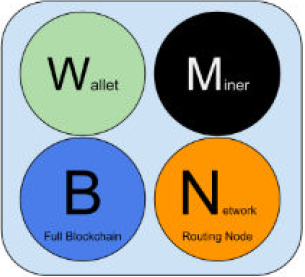
\includegraphics[width=4cm]{imagenes/introduccion/nodo_bitcoin}
    \caption{Un nodo de red bitcoin con las cuatro funciones. Fuente: \cite{antonopoulos2014mastering}}
    \label{fig:funciones-nodo}
\end{figure}

\noindent Todos los nodos incluyen funciones de enrutamiento, validan y propagan transacciones y bloques. Los nodos 
completos, también mantienen una copia completa y actualizada de la Blockchain. Se encargan también de verificar de 
forma autónoma y autorizada cualquier transacción sin referencia externa. Los nodos cartera pueden ser parte de un
nodo completo, en este caso suele ser un cliente de bitcoin de escritorio.

\vspace{5mm}

\noindent Algunos nodos mantienen sólo un subconjunto de la cadena de bloque y verifican las transacciones mediante un 
método llamado verificación de pago simplificado. Estos nodos se conocen como SPV o nodos de peso ligero.

\vspace{5mm}

\noindent Los nodos mineros compiten para crear nuevos bloques ejecutando hardware especializado para resolver el 
algoritmo de Proof-of-Work. Pueden ser completos o ligeros.

\vspace{5mm}

\noindent Además de los principales tipos de nodos del protocolo P2P de bitcoin, hay servidores y nodos que ejecutan 
otros protocolos, como los protocolos de piscinas mineras especializadas y los protocolos de acceso a clientes ligeros. 

\newpage

\noindent Aquí están los tipos de nodos más comunes en la red extendida de bitcoin:

\begin{figure}[ht!]
    \centering
    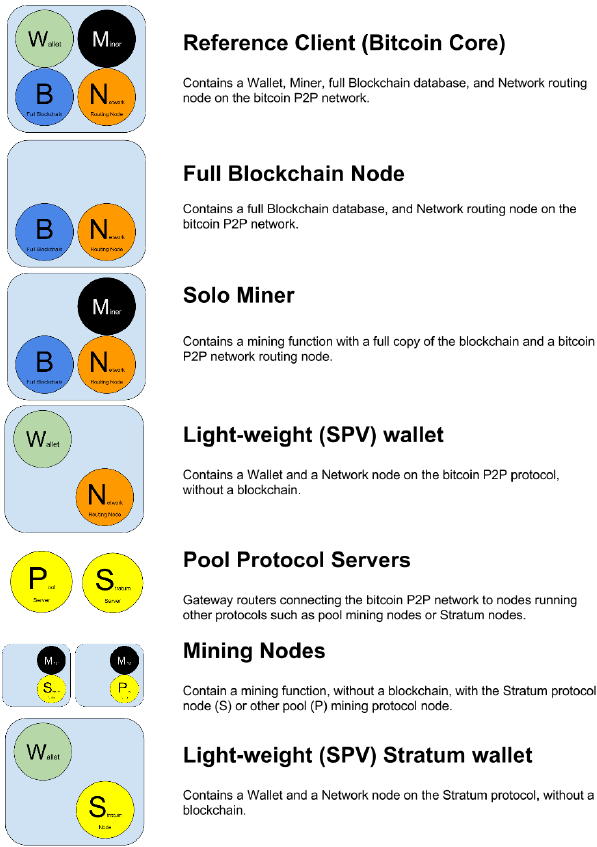
\includegraphics[width=10cm]{imagenes/introduccion/diferentes_nodos_red_extendida}
    \caption{Diferentes tipos de nodos en una red extendida bitcoin. Fuente: \cite{antonopoulos2014mastering}}
\end{figure}

\subsubsection{Blockchain}

La tecnología Blockchain, o también conocido como Distributed Ledger Technology, es una lista ordenada de bloques de 
transacciones vinculados hacia atrás. Cada bloque es identificado por un hash, generado por el algoritmo criptográfico 
SHA256, almacenado en la cabecera del bloque. Cada bloque está enlazado con el anterior bloque (bloque padre) a través 
de su hash en la cabecera del bloque. Dicha secuencia, crea una cadena hasta llegar al primer bloque, conocido como 
el bloque génesis \cite{antonopoulos2014mastering}.

\vspace{5mm}

\noindent Puede darse el caso de que un bloque tenga varios hijos. Los hijos múltiples surgen cuando se produce un fork 
del Blockchain, se debe a que diferentes bloques son descubiertos casi simultaneamente por diferentes mineros. 
Finalmente, un bloque hijo pasa a formar parte del Blockchain y la división se resuelve. 

\vspace{5mm}

\noindent La DLT es inmutable debido a que, en la cabecera del bloque, contiene el hash del padre y, por lo tanto, 
afecta al bloque actual. La identidad del hijo cambia si la del padre también lo hace. Cuando cambia el padre, el 
hash del padre cambia, y por tanto hay que modificar la cabecera del bloque. Esto a su vez cambia el hash del hijo y 
por tanto requiere un cambio en el puntero del nieto y así sucesivamente \cite{antonopoulos2014mastering}.

\vspace{5mm}

\noindent Este efecto de cascada asegura que una vez que un bloque tiene muchas generaciones que lo siguen, no puede 
ser cambiado sin forzar un recálculo de todos los bloques subsiguientes. La existencia de una larga cadena Blockchain 
hace que la historia profunda de la cadena de bloques sea inmutable.

\subsubsection{Minería y consensos}

La minería es la encargada de validar nuevas transacciones, comprobando si son fradulentas, y se registran en el 
libro de contabilidad global. Asimismo, se ocupa de añadir nuevos bitcoins a la oferta monetaria, ya que los 
mineros proporcionan potencia de procesamiento a la red de bitcoin a cambio de la oportunidad de ser recompensados 
\cite{antonopoulos2014mastering}.

\vspace{5mm}

\noindent Cada 10 minutos se \say{extrae} un nuevo bloque que contiene las transacciones que se han producido desde el 
último, añadiendo así esas transacciones a la cadena de bloques. Las transacciones que pasan a formar parte de un bloque 
y se añaden a la cadena de bloques se consideran \say{confirmadas} lo que permite a los nuevos propietarios de bitcoin 
gastar el bitcoin recibido en esas transacciones \cite{antonopoulos2014mastering}.

\vspace{5mm}

\noindent Los mineros pueden recibir dos tipos de recompensas: las creadas por nuevos bloques y tasas de transacciones 
de todas las transacciones dentro del bloque. Para ello, tiene que competir entre ellos para encontrar la solución a 
un problema difícil basado en un algoritmo criptográfico de hash. La solución del problema, llamada Proof-of-Work, 
se incluye en el nuevo bloque y actúa como prueba de que el minero gastó un esfuerzo de computación significativo. 
La competencia por resolver el algoritmo de PoW para ganar recompensas y el derecho a registrar las transacciones 
en la cadena de bloques, es la base del modelo de seguridad de Bitcoin.

\vspace{5mm}

\noindent La minería es el principal proceso de la cámara de compensación descentralizada, por el cual las transacciones 
son validadas y autorizadas. La minería asegura el sistema de bitcoin y permite el surgimiento de consenso en toda la 
red sin una autoridad central \cite{antonopoulos2014mastering}.

\subsubsection*{Consenso decentralizado}

A diferencia de los sistemas de pagos tradicionales, el Bitcoin no tiene una autoridad central sino que cada nodo tiene
una copia completa de un libro de cuentas público como registro de autoridad. Cada nodo de la red comparte la 
información transmitida y, en conclusión, ensamblará una copia del mismo libro público de todos los demás 
\cite{antonopoulos2014mastering}.

\vspace{5mm}

\noindent El consenso descentralizado de Bitcoin surge de la interacción de cuatro procesos que se producen de forma 
independiente en los nodos de la red:

\begin{itemize}
    \item Verificación independiente de cada transacción, por cada nodo completo, sobre la base de una lista completa 
    de criterios
    \item La agregación independiente de esas transacciones en nuevos bloques por nodos mineros, junto con un cálculo 
    demostrado a través de un algoritmo de prueba de trabajo
    \item Verificación independiente de los nuevos bloques por cada nodo y ensamblaje en una cadena
    \item Selección independiente, por cada nodo, de la cadena con el cálculo más acumulativo demostrado a través del 
    PoW
\end{itemize}

\subsubsection*{Algoritmo Proof-of-Work}

La idea de PoW fue publicada por primera vez en 1993 por Cynthia Dwork y Moni Naor, y posteriormente fue 
aplicada por Satoshi Nakamoto en el Bitcoin en 2008 \cite{proof-of-work}. 

\vspace{5mm}

\noindent El problema matemático se puede describir de forma abstracta de la siguiente forma: 

\vspace{5mm}

\noindent \textit{Dados los datos A, encuentra un número x como el que el hash de x adjunto a los resultados de A es un 
número menor que el de B.}

\vspace{5mm}

\noindent La respuesta al problema debe ser un número menor que el hash del bloque para que sea aceptado, conocido como 
el \say{hash del objetivo}. Un hash del objetivo es un número que el encabezamiento de un bloque de hash debe ser igual 
o menor que el de un nuevo bloque, junto con la recompensa, para ser otorgado a un minero. Cuanto más bajo es un 
objetivo, más difícil es generar un bloque \cite{proof-of-work}.

\vspace{5mm}

\noindent El consenso de prueba de trabajo más utilizado se basa en el SHA-256 y se introdujo como parte de Bitcoin.

\vspace{5mm}

\noindent Características del algoritmo: 

\begin{itemize}
    \item Es difícil encontrar una solución para el problema matemático
    \item Es fácil verificar la corrección de esa solución
\end{itemize}

\subsection{Internet de las Cosas (IoT)}

El Internet de las Cosas, o también conocido cómo Internet of Things, consiste en dispositivos que generan procesos, e 
intercambian grandes cantidades de información a través de Internet. Recolectan y comparten datos sobre cómo son 
utilizados y sobre el medio que los rodea. Esta información puede ser utilizada para detertar patrones, hacer 
recomendaciones y detectar posibles problemas antes de que ocurran \cite{what-is-iot, novo2018blockchain}.

\vspace{5mm}

\noindent Desde usos personales como zapatos inteligentes para proveer apoyo al seguimiento y análisis de los datos de 
actitud física, como servicios a la comunidad: control de la cirugía en los hospitales, detectar condiciones 
meteorológicas y proporcionar rastreo y conectividad en los automóviles \cite{khan2018iot}.

\vspace{5mm}

\noindent  Los objetos y sistemas inteligentes permiten automatizar ciertas tareas, especialmente cuando éstas son 
repetitivas, mundanas, requieren mucho tiempo o incluso son peligrosas.

\subsection{La seguridad del Blockchain en IoT}

El uso de la tecnología Blockchain dentro del ambito de los dispositivos IoT, ha tomado un papel importante en la 
gestión, control y seguridad. En esta sección, vamos a describir como la tecnología Blockchain puede ser clave para
proporcionr soluciones de seguridad a los problemas actuales del Internet de las Cosas 
\cite{khan2018iot, reyna2018blockchain}.

\begin{itemize}
    \item \textbf{Espacio de direcciones}: Blockchain tiene 160-bit de espacio de direcciones, a diferencia de IPv6
    que solo tiene 128-bit. Esto es debido a que el hash de la clave pública generada por ECDSA (Elliptic Cruve Digital
    Algorithm) es de 20 bytes o 160-bits. Por lo tanto, podemos alojar alrededor de \(1,46*10^{48}\) direcciones para 
    dispositivos IoT. Lo que hace que sea más escalable a diferencia de IPv6. 
    \item \textbf{Identidad y administración}: Blockchain tiene la capacidad de resolver estos desafíos de manera fácil, 
    segura y eficiente. Se ha utilizado ampliamente para proporcionar un registro de identidad fiable y autorizado, 
    el seguimiento de la propiedad y la supervisión de productos, bienes y activos.
    \item \textbf{Autenticación e integridad de los datos}: Por su diseño, los datos transmitidos siempre estarán
    criptográficamente probados y firmados, garantizando así la autenticación e integridad de los datos.
    \item \textbf{Autenticación, autorización y privacidad}: Provee una solución efectiva en autorización, privacidad en
    los datos y la habilidad de suminstrar reglas de autenticación decentralizada. 
    \item \textbf{Comunicaciones seguras}: Los protocolos que utilizan las IoT son HTTP, MQTT, CoAP o XMPP, y no son 
    seguros por diseño y por tanto, son envueltos por una capa DTLS o TLS. Con Blockchain, la gestión y distribución 
    de claves se elimina totalmente, y cada dispositivo IoT tendrá su par de claves simétricas, para conectarse a la 
    Blockchain.
\end{itemize}

\subsection{¿Qué es una Raspberry Pi?}

La Rasberry Pi es un ordenador de bajo coste hecho por la Raspberry Pi Foundation, del tamaño de una tarjeta de crédito, 
permite aprender programación, construir proyectos de hardware, hacer automatización del hogar, e incluso a nivel 
industrial. Además, tiene la capacidad de interactuar con el mundo exterior, y se ha utilizado en una amplia gama de 
proyectos de creación digital, desde máquinas de música hasta estaciones meteorológicas \cite{what-is-rasp}.

\vspace{5mm}

\noindent El primer modelo lanzado al mercado, tenía una CPU de un solo núcleo de 700MHz y 256MB de RAM 
\cite{what-is-rasp2}, hasta hoy en día que tenemos el modelo 4 con Quad core de 1.5GHz y con diferentes versiones de 
2GB, 4GB y 8GB DDR4 de RAM \cite{rasp-model-4-specifications}.

\vspace{5mm}

\noindent Aunque existen diferentes alternativas, hemos utilizado la Rasberry Pi para este proyecto por comodidad, ya 
que he podido trabajar antes con diferentes modelos de la marca.

\subsection{Conclusión}

En este capítulo hemos dado una introducción al proyecto. Hemos hablado sobre la tecnología Blockchain, apoyandonos 
con el concepto de Bitcoin. Para pasar ha comentar sobre el Internet de las Cosas, y su combinación con el Blockchain, 
También hemos comentado sobre los dispositivos que voy a utilizar como prueba de concepto. A continuación, indagararemos 
más sobre otras tecnologías que han aplicado el Blockchain y plataformas.

\newpage